%%%%%%%%%%%%%%%%%%%%%%%%%%%%
% Intro chapter            %
%%%%%%%%%%%%%%%%%%%%%%%%%%%%

Comme énoncé dans la section \hyperref[chap1:section2]{\textit{\textbf{Problématique}}}, l'AMSN dispose déjà de sondes installées à des points clés des réseaux des OIV. Il s'agit de sondes qualifiées par l'ANSSI et délivrées par une société spécialisée qui fournit également un logiciel permettant d'envoyer directement des règles Suricata aux sondes. Les règles de détection des sondes sont quant à elles mises à jour quotidiennement afin de rester opérationnelles face à l'état de l'art connu de la menace. \\

 Le processus de gestion des sondes préexistant au sein de l'Agence, lorsque j'ai commencé à travailler, était le suivant :\\

\begin{figure}[h]%
    \center%
    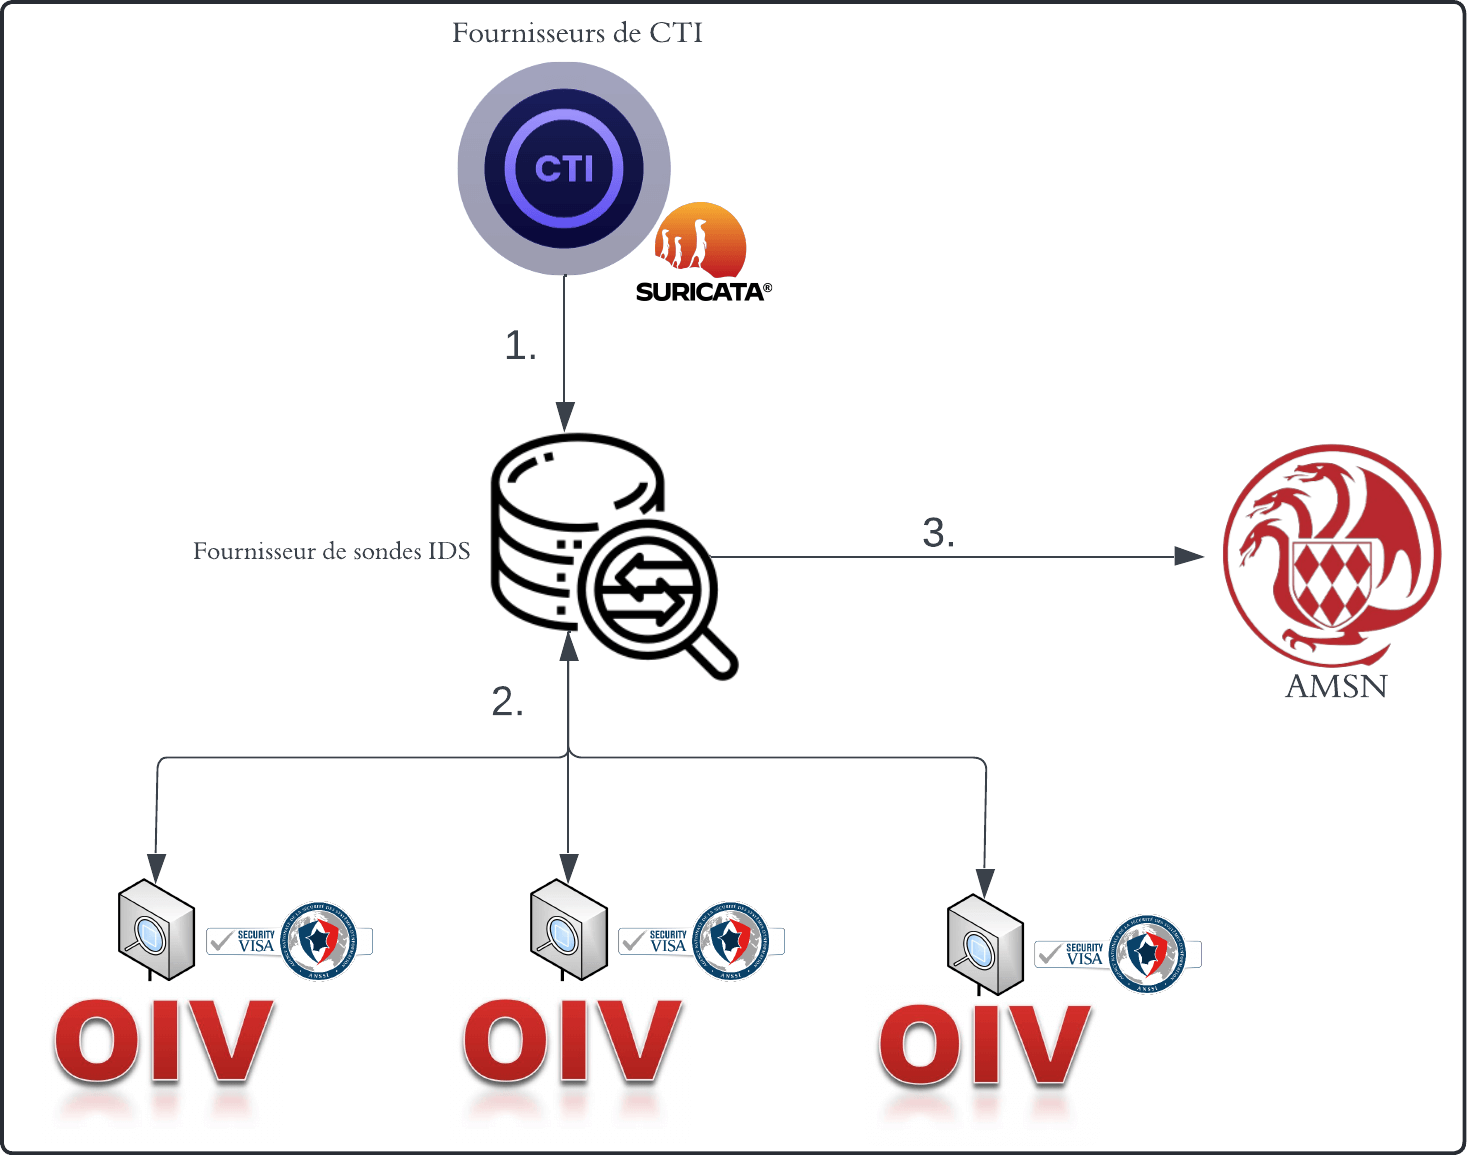
\includegraphics[width=0.73\textwidth]{assets/shemaProcessAMSN.png}
    \caption[Processus d'alimentation des sondes]{Processus d'alimentation des sondes}\label{fig:shemaProcessAMSN}
\end{figure}

\newpage

\begin{enumerate}[itemsep=1em]
    \item L'agence recoit, de la part de partenaires, de la CTI sous la forme de règles Suricata exploitables ;
    \item Les règles sont envoyées au système de gestion des sondes fourni par l'entreprise partenaire spécialisée, qui les distribue aux sondes des OIV ;
    \item Les alertes générées par les sondes sont remontées jusqu'au SOC-MC de l'AMSN.\\
\end{enumerate}

Mon projet professionnel n'a pas profondément modifié ce processus, mais l'a amélioré en s'interposant entre les fournisseurs de CTI et le système de gestion des sondes afin d'améliorer la qualité des règles de détection arrivant finalement dans les sondes IDS.\\

Ce travail d'amélioration s'est organisé en trois grandes étapes :\\

\begin{enumerate}[itemsep=1em]
    \item Création d'un programme automatisé pour contrôler la qualité des règles fournies par les partenaires afin de les filtrer et de les formater avant de les envoyer aux sondes des OIV ;
    \item Mise en place et exploitation d'une instance locale de MISP pour enrichir le programme avec de nouvelles sources de renseignement ;
    \item Exploitation des travaux précédents pour adapter automatiquement les règles envoyées en fonction de l'OIV cible.\\
\end{enumerate}

J'ai réalisé ces différentes missions en suivant la même méthodologie. Tout d'abord, une phase de réflexion était menée conjointement avec mon tuteur de stage et le responsable du SOC-MC pour identifier les attendus du travail à produire. Puis, une phase de développement et de test s'ensuivait pour correspondre à ces attentes. Pour conclure par une phase de rédaction de documentation et de mise en place de tests unitaires afin de permettre la continuité de mon travail sur le temps et sa potentielle prise en main par d'autres personnes.